\renewcommand{\baselinestretch}{1.0}
\chapter{Integration of behaviors: Obstacle Avoidance and Target Acquisition (linear)}%
\label{ch:obstacle-target-linear}
\renewcommand{\baselinestretch}{1.5}
In this chapter the obstacle avoidance and target acquisition behaviors are
integrated, but for the latter is considered a linear dynamic system. The main
differences in the dynamics and corresponding behavior are discussed. Finally,
the best dynamic system form for target acquisition behavior --- nonlinear or linear --- is discussed.

\section{Implementation}%
\label{sec:implementation-obs-tar-linear}
The implementation of the dynamic system that controls the heading direction is
yielded by replacing the nonlinear dynamic system for target acquisition
--- $f_{tar}(\phi)$ --- for the
linear one, as given by Eq.~(\ref{eq:19}), in Eq.~(\ref{eq:36}).

\section{Simulation}
In this scenario, \texttt{MobileRobotDyn\_Tar\_Obs.ttt}, are performed two
simulations for different gaps between obstacles, namely 0 cm and 50 cm span.

\subsection{No gap (0 cm)}%
\label{sec:no-gap-linear}
In the first simulation (Fig.~\ref{fig:obs-tar-linear-behavioral}), the
obstacles form a wall and the robot is positioned in front of the
obstacles but without the sensors detecting them. 
The stochastic force is not considered and the parameter $\beta _{2}$ is 50.

In the initial moments, the sensors do not detect the wall, so the vector field
of the navigation direction is constituted by an attractor, and the dynamic is
linear, since the repulsive forces are zero and the attraction force is
linear. The 90 degrees fixed point is the attractor and there are no repellers,
the robot moves forward (Fig.~\ref{fig:obs-tar-linear-behavioral-1}).

When obstacles are detected, the repulsion forces appear and their intensity
exceeds the attraction force intensity, so in the direction of navigation 90
degrees, a repeller is established. Given the mathematical nature of the
repulsive forces, two attractors are placed, one on the right and the other on
the left, identifying the two directions of escape from the obstacle, (Fig.~\ref{fig:obs-tar-linear-behavioral-2}).

In Figs.~\ref{fig:obs-tar-linear-behavioral-3}
and~\ref{fig:obs-tar-linear-behavioral-4} the robot turns around itself, and
proceeds the navigation direction to one of the attractors, in this case, it
turns right.
The robot continues to circumvent the obstacle until the sensors stop detecting
it, so the behavior falls back to the initial one and the robot reaches the
target (Figs.~\ref{fig:obs-tar-linear-behavioral-5} and~\ref{fig:obs-tar-linear-behavioral-6}).

\begin{figure}[htb!]
  \centering
  \begin{subfigure}{.45\textwidth}
  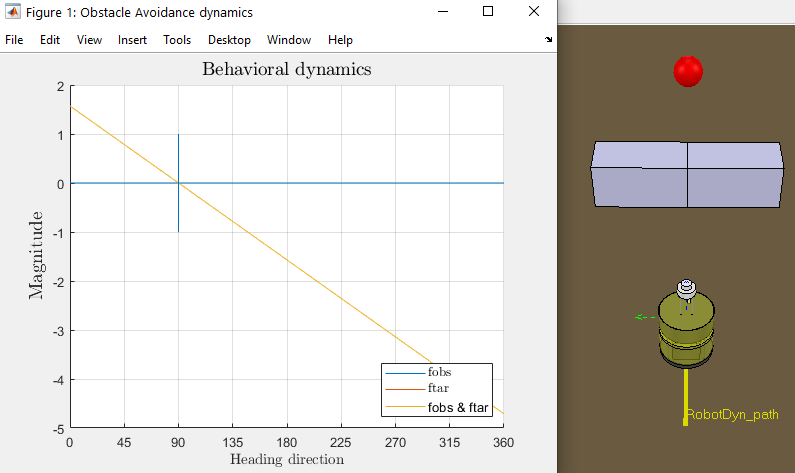
\includegraphics[width=\textwidth]{img/4-1.PNG}%
  \caption{}%
%
  \label{fig:obs-tar-linear-behavioral-1}
  \end{subfigure}
  \begin{subfigure}{.45\textwidth}
    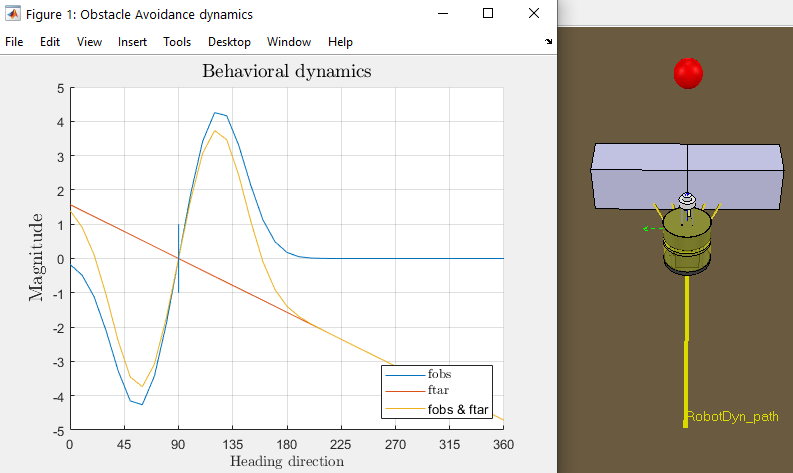
\includegraphics[width=\textwidth]{img/4-2.PNG}%
  \caption{}%
  \label{fig:obs-tar-linear-behavioral-2}
  \end{subfigure}
  % 
  \begin{subfigure}{.45\textwidth}
    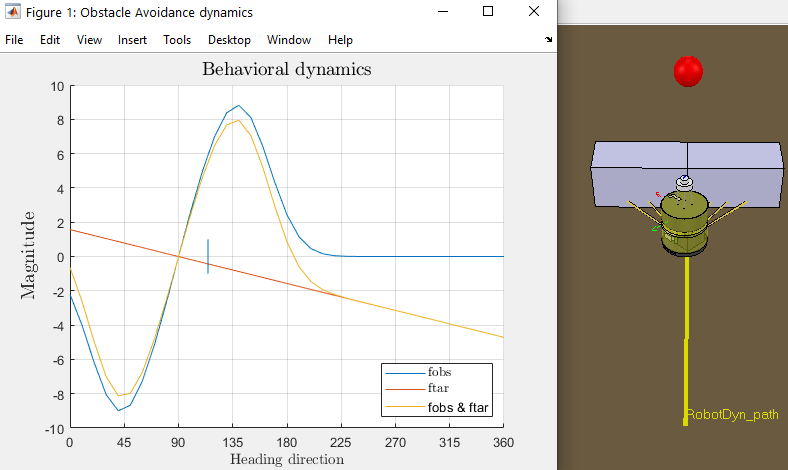
\includegraphics[width=\textwidth]{img/4-3.PNG}%
  \caption{}%
  \label{fig:obs-tar-linear-behavioral-3}
  \end{subfigure}
  % 
  \begin{subfigure}{.45\textwidth}
    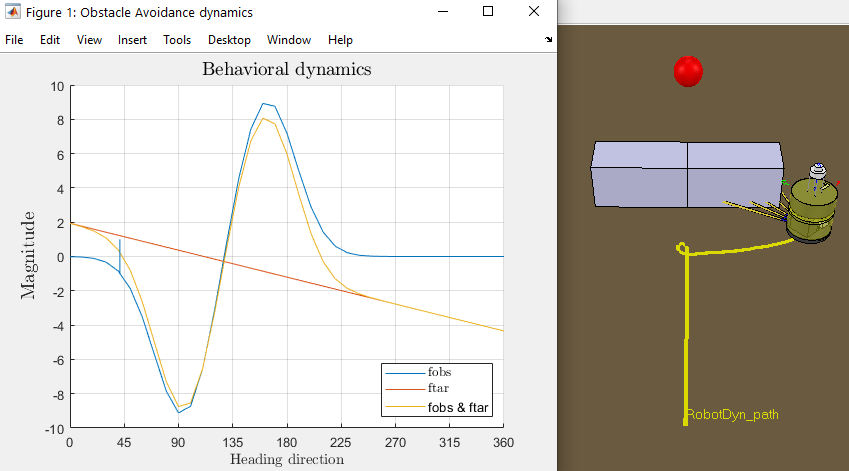
\includegraphics[width=\textwidth]{img/4-5.PNG}%
  \caption{}%
  \label{fig:obs-tar-linear-behavioral-4}
  \end{subfigure}
  \begin{subfigure}{.45\textwidth}
    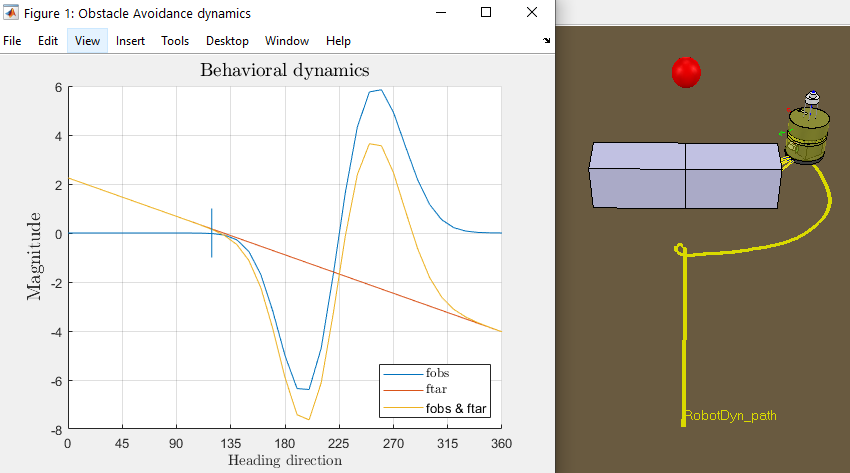
\includegraphics[width=\textwidth]{img/4-6.PNG}%
  \caption{}%
  \label{fig:obs-tar-linear-behavioral-5}
  \end{subfigure}
  % 
  \begin{subfigure}{.45\textwidth}
    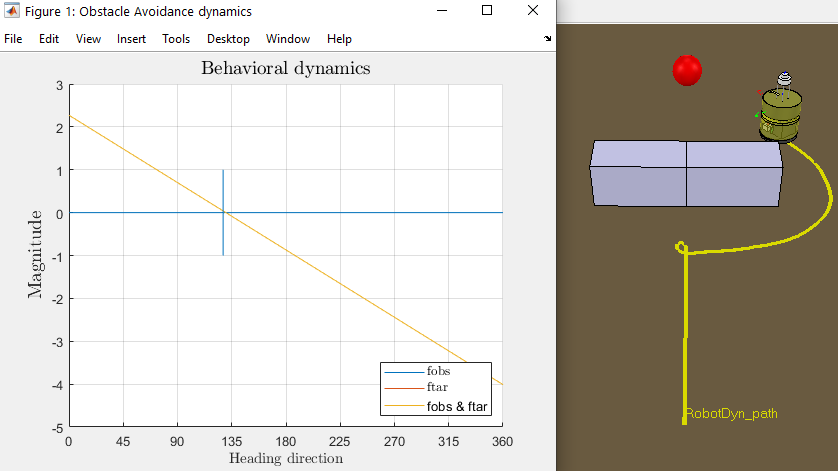
\includegraphics[width=\textwidth]{img/4-7.PNG}%
  \caption{}%
  \label{fig:obs-tar-linear-behavioral-6}
  \end{subfigure}
  \caption{Behavior of the linear system at no gap between obstacles.}%
  \label{fig:obs-tar-linear-behavioral}
\end{figure}

\subsection{50 cm}%
\label{sec:no-gap-linear-50}
A second experiment was carried out in the same scenario and with the same
parameters in which the robustness of both systems, linear and non-linear, were
evaluated (see Fig.~\ref{fig:obs-tar-linear-50} and Video \href{run:./videos/obs-tar-linear.mp4}{./videos/obs-tar-linear.mp4}). 
Both reached the target through the shortest path between obstacles. However,
the linear system showed more abrupt direction adjustments.

\begin{figure}[htb!]
  \centering
%
  \begin{subfigure}{.41\textwidth}
  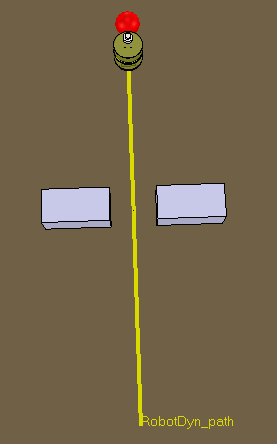
\includegraphics[width=\textwidth]{img/linear.PNG}%
  \caption{Linear}%
  \label{fig:obs-tar-linear-50-1}%
  \end{subfigure}
%
  \begin{subfigure}{.45\textwidth}
    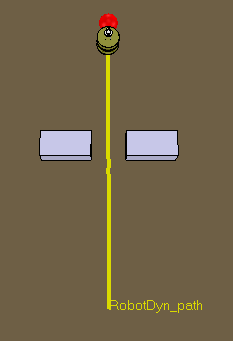
\includegraphics[width=\textwidth]{img/nonlinear.PNG}%
  \caption{Nonlinear}%
  \label{fig:obs-tar-linear-50-2}%
  \end{subfigure}
  % 
    \caption[Comparison of linear and nonlinear dynamic systems for target
    acquisition in the overall dynamics]{Comparison of linear and nonlinear dynamic systems for target
      acquisition in the overall dynamics at a 50cm gap between obstacles}%
    \label{fig:obs-tar-linear-50}%
\end{figure}

\section{Discussion}
After analyzing the robot's behavior for both nonlinear and linear dynamics, it
is now possible to compare them.
Mathematically, the fact that the nonlinear function is a sinusoidal function, yielding always
two fixed points --- one attractor, and in the opposite direction a
repeller --- whereas the linear function only contributes with one attractor to
the vector field. 
The repeller in the opposite direction to the target reinforces the heading direction that must be taken by the robot so that it reaches the target.
In the previous experiments, as well by Section~\ref{sec:discussion-linear-phi},
it is concluded by experimentation too, that the nonlinear system provides smoother paths at narrower angular velocity range.
Thus, it can be concluded that the nonlinear dynamic system is better for the target acquisition behavior of the robot. 

%%% Local Variables:
%%% mode: latex
%%% TeX-master: "../../dissertation"
%%% End:
